\section{Rappresentazione della Conoscenza}
Generalmente la conoscenza musicale di ogni musicista, cantante,
compositore o direttore d'orchestra è formata da tre 
componenti fondamentali:
\begin{enumerate}
\item esecuzioni passate dell'artista stesso
\item esecuzioni altrui ascoltate precedentemente
\item regole provenienti dalla teoria musicale
\end{enumerate}

In IMprovEEsation queste informazioni sono alla base del modello della
conoscenza degli agenti del sistema. Le componenti 1 e 2 costituiscono i
pattern musicali e le relative note associate ad essi. Inoltre nella memoria
degli agenti sono presenti informazioni aggiuntive, come ad esempio
scale, modo degli accordi, etc. Quest'ultime vengono messe in relazione
con i pattern e le note formando così la terza componente, ovvero l'insieme 
di regole teoriche possedute dall'agente.\\ 
Inoltre la conoscenza degli agenti viene rappresentata come se fosse 
immagazzinata in un unica memoria collettiva, che viene acceduta però in
regioni diverse in base al ruolo dell'agente. Ad esempio il direttore ha
accesso alla regione della memoria dove sono salvate le informazioni
riguardo all'andamento complessivo di un improvvisazione che comunicherà
durante quest'ultima ai musicisti. Un agente musicista ha accesso alla
regione di memoria dove salvate le informazioni necessarie per comporre
in tempo reale delle note che siano coerenti in qualche modo con le
informazioni fornite dal direttore.
\subsection{Pattern e Regole}
% XXX MATTE XXX %
Definiamo i pattern come sequenze di misure di accordi. 
Il direttore ha la conoscenza di una collezione di diversi pattern che
a loro volta possono ammettere delle varianti di dinamica e stile.
%TODO: spiegare meglio la struttura del pattern %
Il musicista, nella memoria complessiva, ha accesso alle collezioni di
informazioni riguardo note singole. 
Si è scelto di rappresentare una singola nota come una semicroma essendo 
1/16 la suddivisione temporale più piccola che prendiamo in considerazione.
Inoltre ad ogni semicroma non è associato un solo valore tonale, ma un
vettore di probabilità di dimensione $n$ pari a 13. L'indice i-esimo
di ogni elemento corrisponde alla distanza tonale dalla tonalità decisa
dal direttore, oppure una pausa. Ogni elemento i-esimo del vettore 
corrisponde al valore di probabilità $p_i$ che la nota di distanza 
$i$ dalla tonalità corrente venga selezionata ad un certo istante di tempo $t$. 
Per ogni semicroma è associato anche un valore di probabilità $p_c$
utilizzato per decidere se quella semicroma e il suo vettore di
probabilità debba essere considerato ad un certo istante di tempo $t$.
Nella memoria del musicista sono presenti anche i quarti che raggrupprano 
fino a 4 semicrome ognuno. Ai quarti sono correlate ulteriori informazioni, utili
a comprendere il contesto di appartenenza di un certo quarto, come:
\begin{itemize}
\item posizione del quarto in una misura
\item l'accordo associato
\item il modo dell'accordo 
\item strumento associatio
\item dinamica del quarto
\item mood (stile) del quarto
\item se lo strumento associato è solista o meno
\end{itemize}
Mettendo in relazione queste informazioni con quelle fornite dal
direttore durante un improvvisazione, un musicista cerca di 
scegliere delle note che siano il più possibile inerenti al contesto.
Come ciò viene fatto verrà spiegato nella sezione \ref{thinking}.
\subsection{Database Relazionale}
% XXX MATTE XXX %
\begin{figure}[H]
\centering
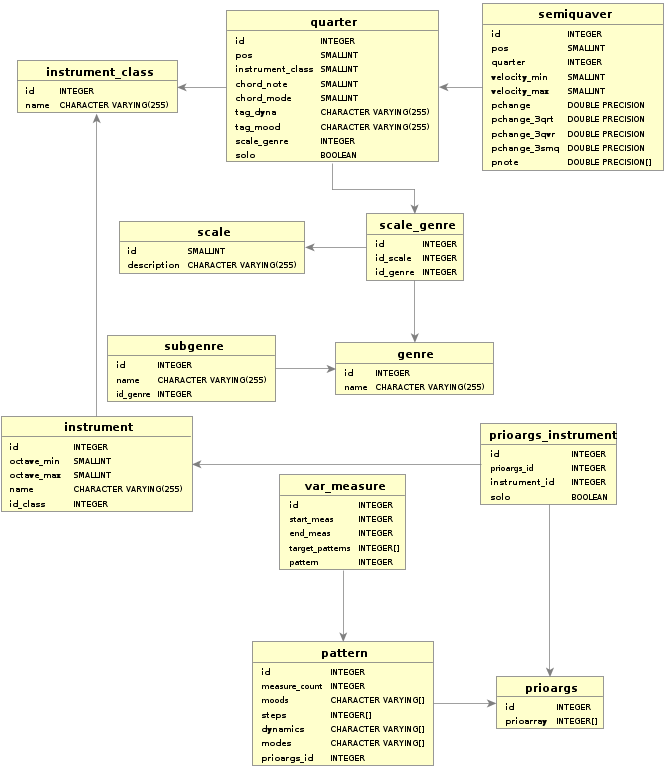
\includegraphics[scale=0.7]{img/db.png}
\caption{Schema E-R del DataBase}
\end{figure}
